\section{Methodology}
In this section, we first describe the datasets employed and the integration of complementary protein features derived from GO, covering both binary and embedding-based representations. We then introduce the architectural framework of the YYYY method and provide an in-depth analysis of its individual components.

\subsection{PPI Networks and Gold Standard}

In this study, we evaluated our proposed method using five PPI networks: Collins, Krogan-Core, Krogan-14K, BioGRID, and the Database of Interacting Proteins (DIP). These networks represent Saccharomyces cerevisiae, a species widely utilized in previous research, providing a baseline for comparative analysis. While most networks include pre-defined interaction weights, BioGRID and DIP do not; we computed weights for these using the cosine similarity of their GO binary feature vectors. For ground-truth validation, we employed the gold-standard reference complexes from multiple biological databases, including MIPS, CYC2008, Aloy, SGD, and TAP06, following the collection criteria established by AdaPPI. We filtered these complexes to include only modules containing at least three proteins. Table \ref{table:dataset-stats} summarizes the statistics for each dataset.

\subsection{Complementary Biological Features}
As complementary biological information, we considered two GO-based protein feature representations: a binary representation and an embedding-based representation. Let \(n\) denote the number of proteins in a given dataset, and let \(m\) represent the total number of GO terms associated with at least one protein across the three GO namespaces, namely BP, MF, and CC. The binary feature vector of protein \(i\) is defined as \(x_i \in \{0,1\}^m\), where \(x_{ij} = 1\) indicates that protein \(i\) is annotated with GO term \(j\), and \(x_{ij} = 0\) otherwise.
The second feature type is an embedding-based representation of GO terms, obtained by applying the Node2Vec algorithm to the GO-basic graph, which yields a \(d\)-dimensional vector for each GO term. Since the embeddings are learned separately for each namespace, the GO term embeddings associated with each protein are first averaged within each sub-ontology, i.e., BP, MF, and CC, and then concatenated to form a \(3d\)-dimensional feature vector.

\begin{table*}[t]
	\centering
	\caption{Statistical summary of the PPI datasets used in this study}
	\label{table:dataset-stats}
	\vspace{2mm}
	\renewcommand{\arraystretch}{1.2}
	\resizebox{\textwidth}{!}{
		\begin{tabular}{lcccccc}
			\toprule
			\textbf{Dataset} & \textbf{Number of Proteins} & \textbf{Number of Interactions} & \textbf{Binary Feature Dimension} & \textbf{Embedding Feature Dimension} & \textbf{Average Degree} & \textbf{Maximum Degree} \\
			\midrule
			Collins & 1622 & 9074 & 2248 & 384 & 11.189 & 127 \\
			Krogan Core & 2708 & 7123 & 3529 & 384 & 5.261 & 141 \\
			Krogan Extended & 3672 & 14317 & 4261 & 384 & 7.798 & 213 \\
			DIP & 4928 & 17201 & 4714 & 384 & 6.981 & 283 \\
			BioGRID & 5640 & 59748 & 4986 & 384 & 21.187 & 2570 \\
			\bottomrule
		\end{tabular}
	}
\end{table*}

\begin{figure*}[t]
	\centering
	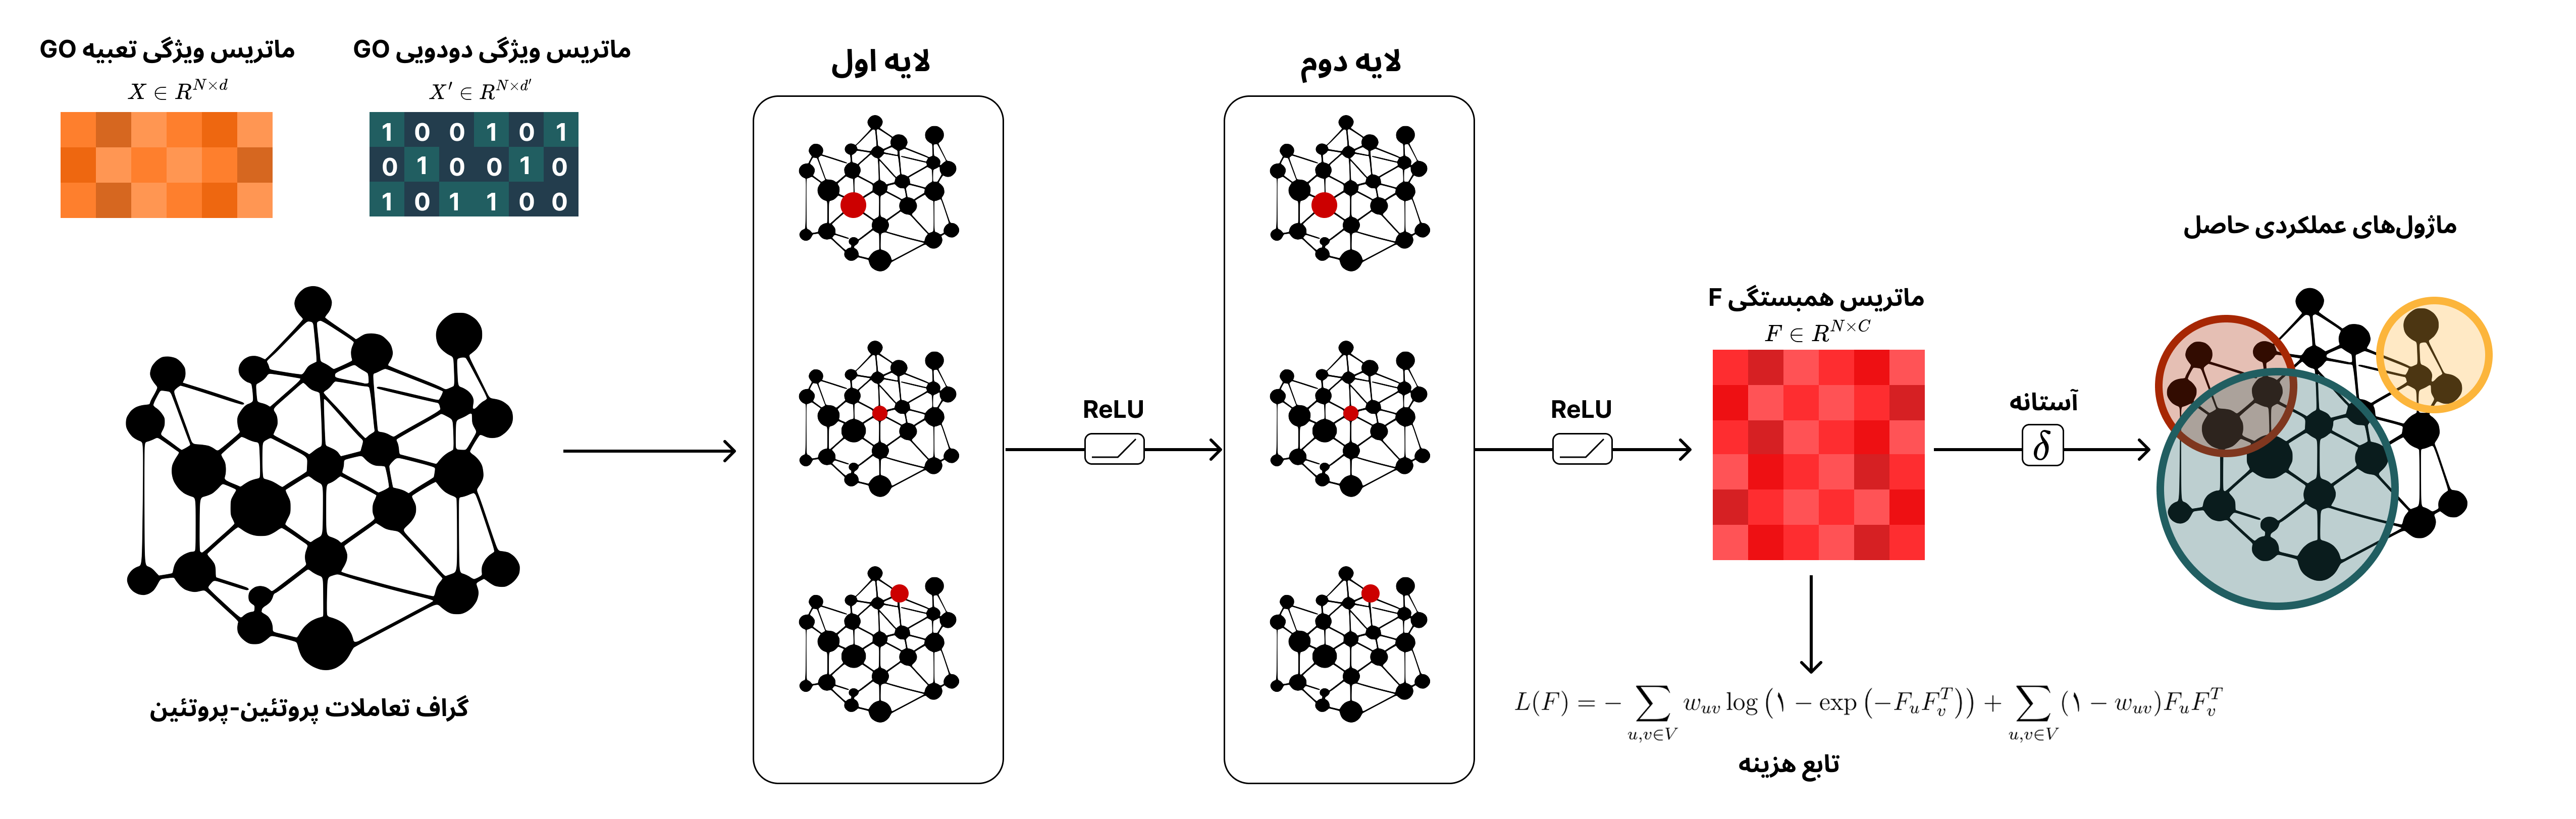
\includegraphics[width=\textwidth]{figures/overall-architecture.png}
	\caption{Overall architecture of the proposed method. The framework integrates protein--protein interaction network information with complementary Gene Ontology-based features to identify functional modules.}
	\label{fig:overall-architecture}
\end{figure*}

\subsection{Overall Architecture}
The overall architecture of the proposed method is illustrated in Figure \ref{fig:overall-architecture}. First, two Graph Attention Networks are trained separately using the binary GO features \(X_B \in \mathbb{R}^{n \times m}\) and the embedding-based GO features \(X_E \in \mathbb{R}^{n \times 3d}\). The proposed loss function is employed for training, while overlapping modularity(defined as equation \ref{eq:modularity-overlapping}) is used as the model selection criterion, resulting in the two trained models \(M_B\) and \(M_E\), respectively. Next, an aggregated thresholding strategy is applied to the affinity matrix produced by each model in order to extract functional modules. Finally, the functional modules identified by the two models, \(M_B\) and \(M_E\), are merged to generate the final set of predicted functional modules.

\subsection{Graph Attention Network}
A Graph Attention Network (GAT) is a type of graph neural network in which, during the aggregation step of message passing, neighboring nodes are not treated equally. Instead of applying a simple aggregation operation, such as the mean used in Graph Convolutional Networks (GCNs), each neighboring node is assigned a learnable attention weight that determines its contribution to updating the representation of the target node. Let \(h_i^{(k)}\) denote the embedding of node \(i\) at the \(k\)-th layer, with \(h_i^{(0)} = x_i\). Then, the embedding at layer \(k+1\) is computed according to Equation \ref{eq:gat-multi}, where \(M\) denotes the number of attention heads, \(\Vert\) represents the concatenation operation, \(N(i)\) denotes the set of neighbors of node \(i\), \(\alpha_{ij}^{(m)}\) denotes the attention coefficient between nodes \(i\) and \(j\) for head \(m\), and \(W^{(m)}\) denotes the learnable weight matrix associated with head \(m\).
\begin{equation}
	h_i^{(k+1)} = \big\Vert_{m=1}^M \sigma\Big(\sum_{j \in \mathcal{N}(i)} \alpha_{ij}^{(m)} W^{(m)} h_j^{(k)} \Big)
	\label{eq:gat-multi}
\end{equation}
The attention coefficient for each head is computed according to Equation \ref{eq:gat-attention-coeff}.

\begin{equation}
	\alpha_{ij}^{(m)} =
	\frac{
		\exp\left(
		\mathrm{LeakyReLU}\left(
		\left(a^{(m)}\right)^T
		\left[
		W^{(m)}h_i^{(k)} \,\|\, W^{(m)}h_j^{(k)}
		\right]
		\right)
		\right)
	}{
		\sum_{n \in \mathcal{N}(i)}
		\exp\left(
		\mathrm{LeakyReLU}\left(
		\left(a^{(m)}\right)^T
		\left[
		W^{(m)}h_i^{(k)} \,\|\, W^{(m)}h_n^{(k)}
		\right]
		\right)
		\right)
	}
	\label{eq:gat-attention-coeff}
\end{equation}




In the proposed method, a two-layer GAT architecture is employed, with each layer followed by a ReLU activation function. In both layers, the input features are mapped to a 512-dimensional space, and the final output is an affinity matrix \(F \in \mathbb{R}^{n \times C}\).
\subsection{Loss Function}

The loss function used in this study is based on NOCD loss as defined in Equation \ref{eq:loss-nocd}. We proposed two versions of NOCD namely Higher Order NOCD (HO-NOCD) and Weighted NOCD(W-NOCD). Considering the $F \in R^{n \times C}$ be the affinity matrix resulted from GAT with parameters $\theta$ as Equation \ref{eq:affinity-matrix}:

\begin{equation}
	F = GAT_{\theta}(X,A)
	\label{eq:affinity-matrix}
\end{equation} 



\textbf{HO-NOCD} The first variant of the proposed loss function, termed HO-NOCD, is motivated by the observation that many proteins within the same complex are not necessarily directly connected in the PPI network. 
% This sentence should be examfact checked through experiments on graph
Instead, the shortest path between two proteins in a complex is often of length two or three. 
In particular, second-order relationships are considerably more common. Therefore, rather than using the first-order adjacency matrix \(A\) and forcing the learned embeddings to reconstruct only direct interactions, it is more appropriate to incorporate higher-order connectivity information into the learning process. To achieve this, the second-order adjacency matrix \(A^2 = AA\) is computed and subsequently thresholded to obtain a binary adjacency matrix, as defined in Equation \ref{eq:nocd-A2}.

\begin{equation}
	\hat{A}_{ij} =
	\begin{cases}
		1 & \text{if } \; \; A^2_{ij} > 0, \\
		0 & \text{otherwise}
	\end{cases}
	\label{eq:nocd-A2}
\end{equation} 

This modification enables the model to capture indirect yet biologically meaningful interactions during the learning process. To balance the contributions of direct and indirect interaction information, the final HO-NOCD loss function is formulated as a convex combination of the first-order and second-order objectives, as shown in Equation \ref{eq:nocd-A2-convex}:

\begin{equation}
	L(F) = (1-\lambda)\, L_{A}(F) + \lambda\, L_{\hat{A}}(F)
	\label{eq:nocd-A2-convex}
\end{equation}

where \(\lambda \in (0,1)\) is a hyperparameter that controls the relative contribution of first-order and second-order structural information in the loss function. Also, the $L_A(F)$ denotes the NOCD loss function which is defined by Equation \ref{eq:loss-nocd} or \ref{eq:loss-nocd-normalized}. This formulation provides sufficient flexibility to capture different structural characteristics across diverse networks.

\textbf{W-NOCD} The second variant of NOCD proposed in this study incorporates interaction weights into the loss function. The main motivation behind this formulation is to account for the confidence and strength of interactions in PPI networks. By incorporating edge weights, the model can better reflect the reliability of observed interactions and reduce the influence of noisy or weak connections, which may otherwise negatively affect the performance of functional module identification.

To incorporate interaction weights into the loss function, Equation \ref{eq:loss-nocd} is modified as shown in Equation \ref{eq:loss-weighted-nocd}. In this formulation, \(w_{uv} \in [0,1]\) represents the weight or confidence of the interaction between proteins \(u\) and \(v\). If no interaction exists between proteins \(u\) and \(v\), the corresponding weight \(w_{uv}\) is set to zero.

\begin{equation}
	L(F) = -\sum_{u,v \in V} w_{uv} \log\left(1-\exp\left(-F_u F_v^T\right)\right)
	+ \sum_{u,v \in V} (1-w_{uv}) F_u F_v^T
	\label{eq:loss-weighted-nocd}
\end{equation}

In Equation \ref{eq:loss-weighted-nocd}, interactions with higher weights contribute more significantly to the loss function, while interactions with low or zero weights have a smaller influence. As a result, the model focuses more on reliable and biologically meaningful interactions while reducing the impact of weak or noisy connections. In contrast, the original NOCD loss function treats all interactions equally regardless of their reliability. By explicitly accounting for interaction strength, the proposed weighted formulation can improve the accuracy of functional module identification.


\subsection{Aggregating Thresholding and Protein Complex Extraction}

Let \(M_B\) and \(M_E\) denote the GAT models trained using the input feature sets \(X_B\) and \(X_E\), respectively, resulting in the corresponding representation matrices \(F_B\) and \(F_E\). Unlike the original NOCD method, which employs a single threshold for community extraction, the proposed approach utilizes multiple thresholds in the range \(\{0.2, 0.3, \dots, 0.7\}\). The primary motivation behind this strategy is the highly overlapping nature of protein complexes. As illustrated in Figure \ref{}, proteins may participate in multiple complexes simultaneously, and therefore a single threshold may fail to capture complexes with different structural densities.

Let \(K_{\phi}(F)\) denote the set of protein complexes extracted from representation matrix \(F\) using threshold \(\phi\). The final sets of extracted complexes are obtained according to Equation \ref{eq:extract_subsets}.

\begin{equation}
	\begin{split}	
		S_B &= \bigcup_{\phi \in \{0.2,0.3,\dots,0.7\}} K_{\phi}(F_B) \\
		S_E &= \bigcup_{\phi \in \{0.2,0.3,\dots,0.7\}} K_{\phi}(F_E) \\
		S &= S_B \cup S_E
	\end{split}
	\label{eq:extract_subsets}
\end{equation}

Considering the fact that sets do not contain duplicated elements, we use sets notation to model our extracting protein complexes process. in Equation \ref{eq:extract_subsets}, \(S_B\) and \(S_E\) represent the sets of protein complexes extracted from the binary GO feature model and the embedding-based GO feature model, respectively. For each model, complexes identified across different threshold values are aggregated using the union operation in order to capture complexes with varying levels of cohesiveness and overlap. Finally, the outputs of both models are merged to construct the final set of predicted protein complexes, denoted by \(S\).




